\section{Introduction}

Over the last few years, pre-trained models have greatly revolutionized computer vision (CV) and natural language processing (NLP). 
The first wave of exploring pre-trained models took place in the field of CV. Deep convolutional neural nets~\citep{krizhevsky2012imagenet, simonyan2014very, he2016deep} are pre-trained on well-labeled  ImageNet~\citep{deng2009imagenet} and then transferred to downstream CV tasks~\citep{girshick2014rich, long2015fully, vinyals2015show}.
Standardly, CV models are pre-trained to predict a fixed set of pre-defined object categories, e.g., 1000 classes in ImageNet.
However, this supervised pre-training is hard to scale since we need arduous human labeling to specify new visual concepts.
% Notwithstanding the unprecedented performance, CV models are pre-trained to predict a fixed set of pre-defined object categories, e.g., 1000 classes in ImageNet, which dramatically limits their generality and scalability since we need arduous human labeling to specify new visual concepts. 
% When pre-training meets NLP, the intrinsic supervision within the natural language makes the pre-training more scalable~\citep{devlin2018bert, radford2019language, brown2020language}.
%More specifically, benefiting from task-agnostic objectives such as autoregressive~\citep{yang2019xlnet} and Masked Language Model (MLM)~\citep{devlin2018bert}, the performance can be steadily improved via scaling up the data, model capacity, and computation~\citep{brown2020language, fedus2021switch}.
%Witnessing this progress in NLP, we try to answer the following question in this paper: \textit{could we use broader and scalable supervision to learn visual representations?} \wl{(This question seems to be too broad and can also be answered by the method in CLIP. Then this is not the special question we aim at)}
%However, the scaling up for pre-training needs not only more storage space but also expensive computing machines. In the field of computer vision, it is harder to obtain a large number of clean data, and most organizations cannot afford the resources consumed to perform large-scale model pre-training. Witnessing this problem, we try to answer the following question in this paper: \textit{Could we use broader and scalable supervision to learn the general representation and obtain competitive results when there are not sufficient computational resources and prohibitive datasets?}

When pre-training meets NLP, the intrinsic supervision within the natural language makes the pre-training more scalable~\citep{devlin2018bert, radford2019language, brown2020language}. 
Witnessing the progress in NLP, researchers use natural language supervision to learn visual features.
The language-image pre-training can scale up to a very large size, benefiting from abundant image-text pairs on the Internet.
For instance, CLIP~\citep{radford2021learning} and ALIGN~\citep{jia2021scaling} adopt the contrastive loss to push the embedding of matched image-text pairs together while pushing those of non-matched pairs apart. They achieve prestigious performance by learning from an enormous dataset that contains 400M/1B image-text pairs. 
However, these methods also require huge storage and computing resources, which is not affordable for most laboratories and companies. 
We argue that these prior arts only use the single image-text contrastive supervision while overlooking the widespread supervision within the pairs, thus is inefficient.
% We argue that these prior arts only use the single image-text contrastive supervision, thus is inefficient. 
% while overlooking the widespread supervision within the pairs, which is inefficient. 
% To mitigate this problem, we dig inside into the intrinstic supervisons with the image-text pairs

% Witnessing these problems, we try to answer the following question in this paper: \textit{Could we learn the general representation and obtain competitive results when there are not sufficient computational resources and prohibitive datasets by using broader and scalable supervision?}

% requires tremendous work. \wl{(what do we mean by `tremendous work'?)}, and it is also prohibitive work \wl{(`prohibitive' is too strong here, at least there is some paper achieving this)} to train models on such vast datasets. 
% \checkme{Witnessing this progress in NLP, we try to answer the following question in this paper: \textit{could we use broader and scalable supervision to learn visual representations?} \wl{(This question seems to be too broad and can also be answered by the method in CLIP. Then this is not the special question we aim at)}}

% We argue that these prior arts only use the single image-text contrastive supervision while overlooking the widespread supervision within the pairs, which is inefficient.

% In this paper, we utilize the widespread supervision within the pairs to learn visual representation efficiently.
Firstly, there underlies rich structural information within each modality itself~\citep{lecun2021self}. 
We can tweak some words/pixels in a sentence/image while retaining a similar semantic meaning. 
This sort of self-supervision can be exploited to learn a more common-sense representation for each modality~\citep{devlin2018bert, he2020momentum, chen2020simple}. 
Moreover, inspired by contrasting multi-crops in an image~\citep{caron2020unsupervised}, we further extend the multi-view \footnote[1]{\label{view}View is originally a visual concept. For simplicity, we use the same term for language.} supervision into our multi-modality setting.
Specifically, each image is paired with multiple textual descriptions obtained via stochastic augmentations, vice versa. 
The benefit is intuitive: this auxiliary multi-view supervision brings more invariant and robust information. 

\begin{figure}[t]
    \vspace{-2em}
    \begin{minipage}[t]{0.5\linewidth}
	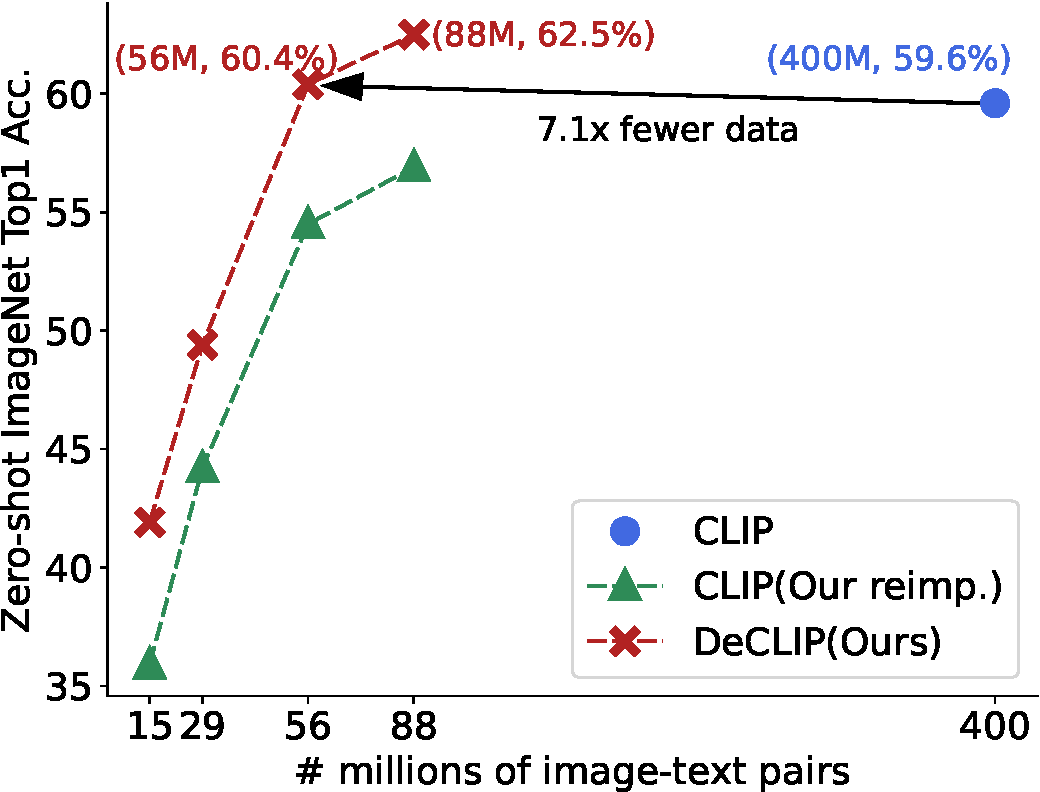
\includegraphics[width=0.99\columnwidth]{DeCLIP/figs/IN_zero_shot.pdf}
	\hspace{-45mm}\resizebox{.6\columnwidth}{!}
	{\tablestyle{2pt}{1}
        \begin{sc}
		\begin{tabular}[b]{l|lllll}
			Data & 15M & 29M & 56M & 88M & 400M \\
			\midrule
			CLIP & 35.9$^\dagger$  & 44.2$^\dagger$ & 54.5$^\dagger$ & 56.9$^\dagger$ & 59.6 \\
			DeCLIP & 41.9  & 49.3 & 60.4 & 62.5 & \# \\
			\multicolumn{6}{l}{~~$^\dagger$ Our reimplementation.}
			\vspace{30mm}
        \end{tabular}
	    \end{sc}}
    \vskip -0.05in
	\caption{
	Zero-shot performance of CLIP-ResNet50 and our \workname-ResNet50 when using different amounts of data. (88M, 62.5\%) denotes the use of 88M data with top-1 accuracy 62.5\% on the ImageNet-1K validation dataset. Our model has much better data efficiency.}
	\label{fig:IN_zero_shot}
	\end{minipage}%
    \begin{minipage}[t]{0.5\linewidth}
	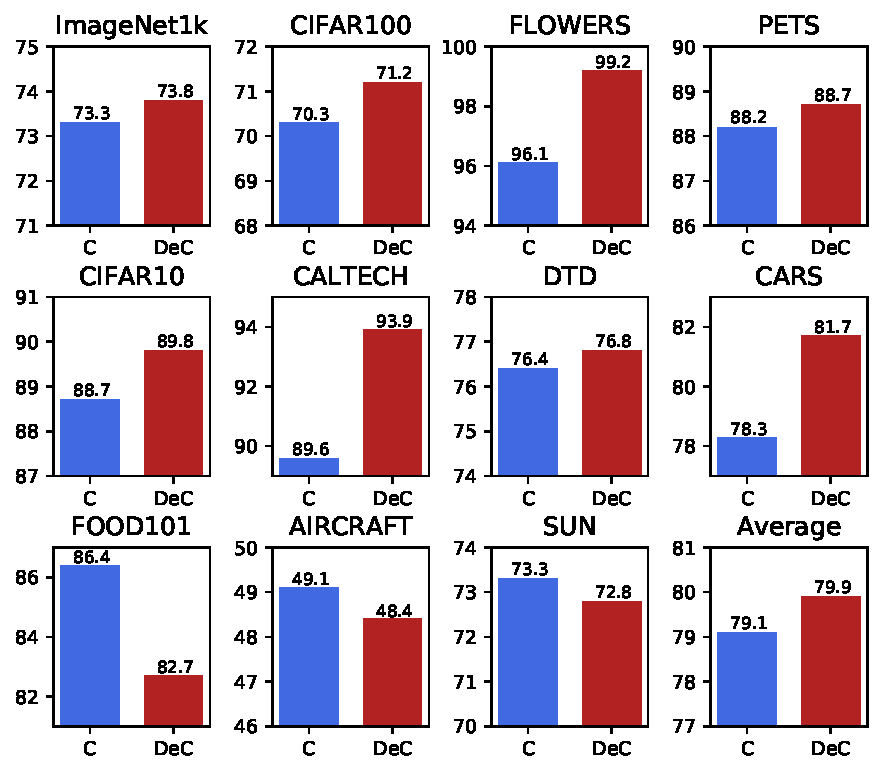
\includegraphics[width=1.0\columnwidth,height=5.5cm]{DeCLIP/figs/downstream_v9.pdf}
	\vskip -0.05in
	\caption{
	Transfer the \workname-ResNet50 (abbr. as DeC) and CLIP-ResNet50 (abbr. as C) to 11 downstream visual datasets using linear probe verification. Our \workname achieves better results in 8 out of 11 datasets. 
	}
	\label{fig:Downstream}
	\end{minipage}%
% 	\vspace{-1em}
\end{figure}




\begin{wrapfigure}{o}{0.35\textwidth}
\vspace{-2em}
    \begin{center}
    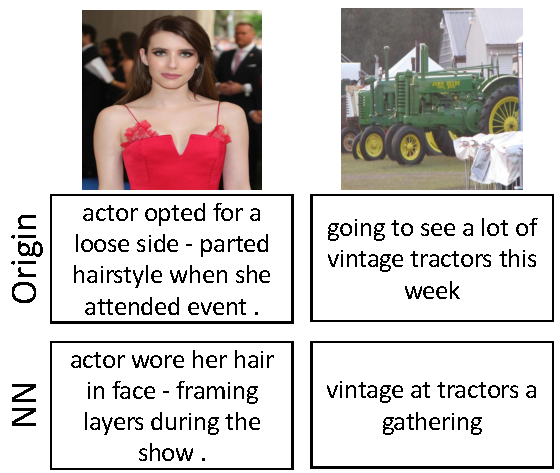
\includegraphics[width=\linewidth]{DeCLIP/figs/CC2image.pdf}
    \end{center}
    \vspace{-1em}
        \caption{Examples of Nearest Neighbor from Conceptual Captions dataset.}
        % \vspace{-0em}
    \label{fig:NN-supervision-small}
        \vspace{-2em}
\end{wrapfigure}

Besides these overlooked supervision, we propose a novel nearest-neighbor (NN) supervision from other similar pairs. This NN supervision is mainly based on the intuition that one image is likely to have other similar text descriptions among the dataset. As shown in right figure, the image with the text \texttt{'going to see a lot of vintage tractors this week'} can also be described by \texttt{'vintage at tractors a gathering'}. For this reason, we sample the NN in the embedding space and utilize them as additional supervisory signals. 
% The NN supervision can also be regarded as a semantic-level augmentation.
Aggregating these supervision leads to our novel training paradigm \workname, which stands for \textbf{D}ata \textbf{e}fficient \textbf{C}ontrastive \textbf{L}anguage-\textbf{I}mage \textbf{P}retraining. 

% \textbf{Thirdly}, since pairs are collected from the Internet, there is considerable noise in the image-text datasets~\citep{thomee2016yfcc100m, sharma2018conceptual}.
% Besides the paired text, one image is likely to have other semantically similar text descriptions among the dataset. 
% For this reason, we sample the nearest neighbors in the embedding space and utilize them as additional supervisory signals. As shown in Fig~\ref{fig:NN-supervision-small}, the nearest-neighbor supervision can be viewed as a semantic-level augmentation or a soft regularization that suppresses the data's noise. 
% % Each of the additional supervision is found to boost the performance of zero-shot representation. 
% Aggregating these supervision leads to our novel training paradigm \workname, which stands for \textbf{D}ata \textbf{e}fficient \textbf{C}ontrastive \textbf{L}anguage-\textbf{I}mage \textbf{P}retraining. 


Extensive experiments show the effectiveness and efficiency of our \workname. As shown in Fig.~\ref{fig:IN_zero_shot}, with a ResNet50 image encoder and a Transformer text encoder, 
our model can achieve 60.4\% zero-shot top1 accuracy on ImageNet, which is 0.8\% above the CLIP-ResNet50 while using 7.1$\times$ fewer data. 
Using only 88M image-text pairs, our best ResNet50/ViT-B32 models boost the zero-shot performance to 62.5\% and 66.2\%, nearly 3.0\% higher than the best number reported for these two architectures. 
We further verify the transferability of our models on downstream tasks.
As indicated in Fig.~\ref{fig:Downstream}, our \workname-ResNet50 outperforms its counterpart in 8 out of 11 visual datasets.
Moreover, Scaling up the model and computing also works well in our framework. 
Using 4.5$\times$ fewer data, our \workname-RegNetY-64GF achieves 73.7\% zero-shot ImageNet top1 accuracy, which is on-pair with CLIP-R50$\times$64.
Pre-trained models, code, and datasets shall be released to the community. The contributions are summarized as follows:

% \paragraph{Summary of contributions.} 

% \begin{itemize}
% \item release stronger baseline for CC/release YTCC15M data and benchmark/release web data query
% \item Stronger Paradigm/2view/ssl/nn
% \item dowstream: aug ploicy
% \end{itemize}




% \begin{figure}[t]
% 	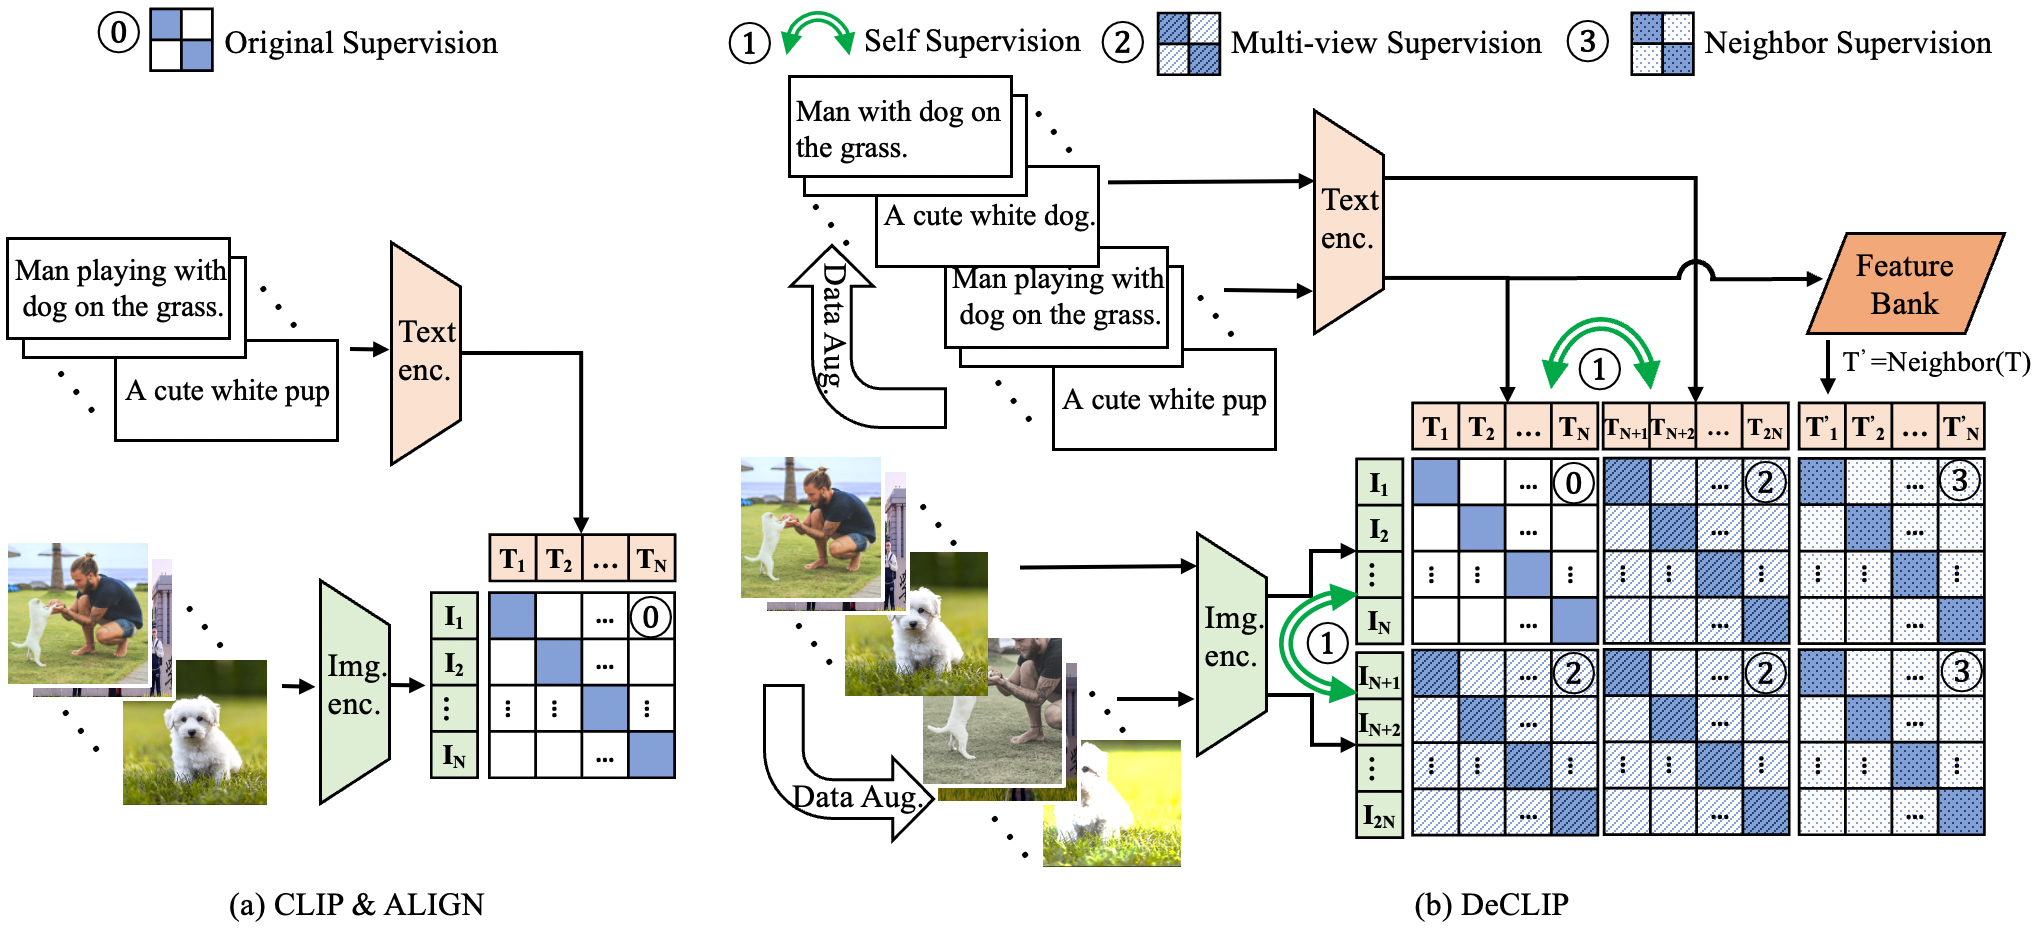
\includegraphics[width=0.99\columnwidth]{DeCLIP/figs/main_figure.png}
%     \vskip -0.15in
% 	\caption{Summary of our DeCLIP.}
% 	\label{fig:IN_zero_shot}
% \end{figure}

% \checkme{The contributions of this work are summarized as follows:}
\begin{itemize}[leftmargin=*]
    % self supervision ? 
    \item 
    % To the best of our knowledge, it is the first work to introduce self-supervision to the million-scale image-text pre-training task.
    To the best of our knowledge, this is the first work to study self-supervision and cross-modal multi-view supervision in the million-scale image-text pre-training task. 
    % Experimentally, these overlooked supervision 
    Our work opens a new direction to fully exploit the intrinsic supervision within the multi-modal data instead of scaling up data naively.
    % \item We introduce the cross-modal multi-view supervision to extract richer and more invariant information within the image-text pair. It is naturally compatible with the image-text contrastive loss, which makes it easy to adopt.
    \item We propose novel cross-modal Nearest-Neighbor Supervision (NNS)  to harness information from other similar pairs. The NNS can also be regarded as a semantic-level augmentation.
    % With nearest-neighbor supervision, we could make full use of the features by learning from other similar text descriptions among the dataset besides its paired text.
    % The NN supervision is based mainly on the intuition that one image is likely to have other high-quality text descriptions among the dataset besides its paired text.
    %\item Instead of scaling up data naively, our work opens up a new direction to fully exploit the intrinsic supervision within the multi-modal data. Experimentally, \workname shows superior effectiveness and efficiency with different types of neural nets(CNN and ViT) and different amounts of data. \wl{(I do not consider this as a contribution)}
    % \item We propose three additional supervision: self-supervision within each modality, cross-modal multi-view supervision, nearest-neighbor supervision from other similar pairs to learn visual representations more effectively and efficiently. \checkme{split it?}
    % \item In order to solve the data-hungry problem of vision language pre-training, We use open source data and crawled data to construct 88M high quality image-text pairs dataset, named \workname-88M. 
    % \item We propose the \workname paradigm, which obtains more supervision from three parts: self-supervision within each modality, multi-view supervision across modalities, and nearest-neighbor supervision from other similar pairs, to learn more general visual representations.
    % \item Extensive experiments show the effectiveness and efficiency of our \workname. we achieve the best ResNet50 and ViT-B/32 models using only 88M image-text pairs, and also provide a small but very effective benchmark for academia and industry.
    % \item \checkme{split it?}
\end{itemize}
